\documentclass{article}

\usepackage{amsmath, physics, gensymb, microtype, float, multicol}
\usepackage{tikz, tikz-3dplot, pgfplots}
\usepackage[letterpaper, bottom=1in]{geometry}

\pgfplotsset{compat=newest}

\newcommand{\dt}{\mathrm{d}t}
\newcommand{\x}{\mathrm{x}}
\newcommand{\y}{\mathrm{y}}
\newcommand{\z}{\mathrm{z}}
\newcommand{\vel}{\mathrm{v}}
\newcommand{\ddt}[1]{\frac{\mathrm{d}#1}{\dt}}
\newcommand{\dydt}{\frac{\mathrm{d}y}{\dt}}

\title{Newton's Law}
\date{2/6/2023}
\author{Laith}

\begin{document}
\maketitle

\hrule
\section{Laws:}

\subsection*{First Law:}
    If an object is not experiencing the effect of any 
    force, then it will either remain stationary \textbf{or}
    keep moving with constant \underline{velocity}.

\subsection*{Second Law:}
    If force $\va{F}$ is acting on an object with 
    mass $m$, then the acceleration $\va{a}$ is given by:
    \[\va{F}=M\va{a}\]
\begin{multicols}{2}
\begin{figure}[H]
    \begin{tikzpicture}
        \draw (0, 0) -- (6, 0);

        \draw[thick] (1, 0) -- (1, 2);
        \draw[thick] (1.5, 0) -- (1.5, 1.5);
        \draw[thick] (4.5, 0) -- (4.5, 1.5);
        \draw[thick] (1.5, 1.5) -- (4.5, 1.5);
        \draw[thick] (1, 0) -- (1.5, 0);
        \draw[thick] (4.5, 0) -- (5, 0);
        \draw[thick] (5, 0) -- (5, 2);
        \draw[thick] (1, 2) -- (5, 2);
        \draw (2, 2) -- (2, 3);
        \draw (4, 2) -- (4, 3);
        \draw (2, 3) -- (4, 3);

        \draw[blue, stealth-stealth] (2.5, 0) node[below] {$Mg$} -- (2.5, 4) node[above] {$N$};

        \node at (3, 2.5) {$M$};
    \end{tikzpicture} 
    \caption{Book on a Table}
\end{figure}

\columnbreak
Since the book is not moving, the net forces (sum of the forces) 
should equal 0 N. Since the forces are vectors, the forces must act 
in opposite directions in order for them to cancel out in addition to 
having the same magnitude. 
Like you can see in the above figure, the normal force $N$ of the table acts upwards, 
which is opposite to the downward acting force of gravity $Mg$. 

Mathematically, this would look like:
\[\sum F_{net} = N+Mg = 0\,\mathrm{N}\]
Generally speaking, \textbf{a net force of 0 N means all 
components of force are 0}:
\[ \va{F}_{net} = (0, 0, 0)\]
\end{multicols}

\hrule
\section{Free-Body Diagrams}
We can use free-body diagrams to model forces:
\begin{multicols}{2}
\begin{figure}[H]
    \centering
    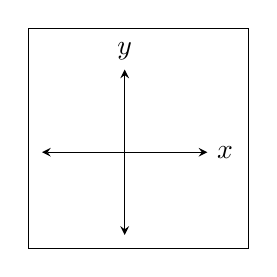
\begin{tikzpicture}[scale=0.35]
        \draw[thin] (-3.5, -3.5) -- (4.5, -3.5) -- (4.5, 4.5) -- (-3.5, 4.5) -- (-3.5, -3.5);
        \draw[stealth-stealth] (0, -3) -- (0, 3) node[above] {$y$};
        \draw[stealth-stealth] (-3, 0) -- (3, 0) node[right] {$x$};
    \end{tikzpicture}
\end{figure}

\columnbreak
\noindent Free-body diagrams can be rotated to match the orientation of the object in question:
where with respect to the object, the vertical force vectors form the $y$-axis and the 
horizontal force vectors form the $x$-axis.
\end{multicols}

\section{Types of Forces}
\begin{enumerate}
    \item $\va{N}$ : Normal force; the force that acts perpendicular to a surface.
    \item $\va{Mg}$ : Gravitational force; the force that acts downwards on an object,
    calculated by multiplying the mass of an object by acceleration due to gravity.
\end{enumerate}
\textbf{\underline{Remark:} acceleration $\va{a}$ is not a force, but it is caused by forces.}
\vspace{1em}

\hrule
\section{Example Problem}

Determine the $x$ and $y$ components of the net force on the box:
\begin{figure}[H]
   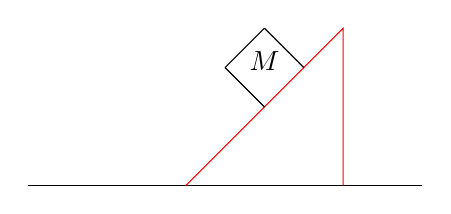
\begin{tikzpicture}
        \draw (0, 0) -- (5, 0);

        \draw[red] (2, 0) -- (4, 2) -- (4, 0);
        \draw (3.5, 1.5) -- (3, 2);
        \draw (3, 1) -- (2.5, 1.5);
        \draw (2.5, 1.5) -- (3, 2) node[below, yshift=-5] {$M$};
        
   \end{tikzpicture} 
\end{figure}

\noindent We can draw a free-body diagram to model the forces acting on the box with mass $M$:
\begin{figure}[H]
    \centering
    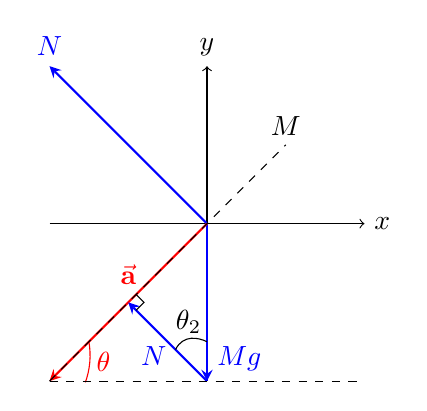
\begin{tikzpicture}
        \draw[->] (-2, 0) -- (2, 0) node[right] {$x$};
        \draw[->] (0, -2) -- (0, 2) node[above] {$y$};

        \draw[thick, blue, -stealth] (0, 0) -- (-2, 2) node[above] {$N$};
        \draw[thick, blue, -stealth] (0, 0) -- (0, -2) node[above right] {$Mg$};
        \draw[thick, red, -stealth] (0, 0) -- (-2, -2) node[midway, yshift=10] {$\va{a}$};
        \draw[thick, blue, stealth-] (-1, -1) -- (0, -2) node[midway, xshift = -5, yshift=-5] {$N$};
        \draw (-0.9, -0.9) -- (-0.8, -1) -- (-0.9, -1.1);
        \draw (0, -1.5) .. controls (-0.1, -1.45) and (-0.3, -1.4) .. (-0.4, -1.6) node[midway, yshift=6, xshift=-1] {$\theta_2$};
        \draw[red] (-1.5, -1.5) arc (10:-20:1) node[midway, xshift=5] {$\theta$};
        \draw[dashed] (-2, -2) -- (2, -2);
        \draw[dashed] (-2, -2) -- (1, 1) node[above] {$M$};
    \end{tikzpicture}
\end{figure}

For the $x$ component, we need to look at the angle $\theta_2$ formed between the 
normal force vector $N$ and gravity vector $Mg$. We can see 
that the vectors form a triangle, which allows us to use the trigonmetric functions 
to setup an equation in which we can solve for $x$.
Since the only force acting horizontally on the box is $Mg$, 
we can just solve for the height of the triangle (the side aligned with the incline) using 
$\sin$.
\begin{align*}
    &\sin(\theta_2) = \frac{x}{Mg} \\ 
    \Rightarrow \, &\boxed{x = \sin(\theta_2)Mg}
\end{align*}
For the $y$ component, there are multiple forces acting in this direction. Thus, we have to 
determine what these forces are and their $y$ components. 

One of these forces is the normal force $N$. With respect to the box, it is only
pushing up on the box. This means that $N$ has a $y$-component, but no $x$-component (or an $x$-component of 0 N).
As a result, the $y$-component of $N$ will be itself (this might not remain true for a 3D space where 
$z$-components exist). 

The next force is $Mg$, since in addition to horizontal force, it also has a vertical force
acting on the box, in which $Mg$ is bring the box to the ground. We can rotate our free-body 
diagram to match the orientation of the box in order to more easily break apart $Mg$ into its 
$x$ and $y$ components:
\begin{figure}[H]
    \centering
    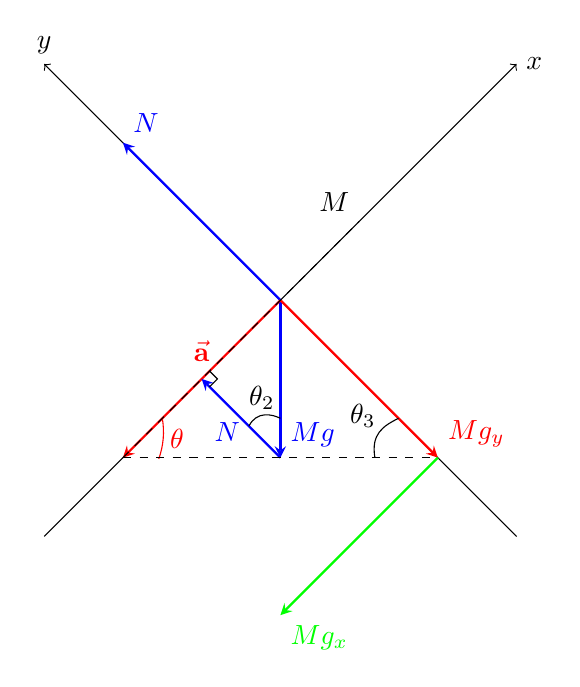
\begin{tikzpicture}
        \draw[->] (-3, -3) -- (3, 3) node[right] {$x$};
        \draw[->] (3, -3) -- (-3, 3) node[above] {$y$};

        \draw[thick, blue, -stealth] (0, 0) -- (-2, 2) node[above right] {$N$};
        \draw[thick, blue, -stealth] (0, 0) -- (0, -2) node[above right] {$Mg$};
        \draw[thick, red, -stealth] (0, 0) -- (2, -2) node[above right] {$Mg_y$};
        \draw[thick, green, -stealth] (2, -2) -- (0, -4) node[below right] {$Mg_x$};
        \draw[thick, red, -stealth] (0, 0) -- (-2, -2) node[midway, yshift=10] {$\va{a}$};
        \draw[thick, blue, stealth-] (-1, -1) -- (0, -2) node[midway, xshift = -5, yshift=-5] {$N$};
        \draw (-0.9, -0.9) -- (-0.8, -1) -- (-0.9, -1.1);
        \draw (0, -1.5) .. controls (-0.1, -1.45) and (-0.3, -1.4) .. (-0.4, -1.6) node[midway, yshift=6, xshift=-1] {$\theta_2$};
        \draw (1.5, -1.5) .. controls (1.3, -1.6) and (1.15, -1.7) .. (1.2, -2) node[midway, yshift=6, xshift=-6] {$\theta_3$};
        \draw[red] (-1.5, -1.5) arc (10:-20:1) node[midway, xshift=5] {$\theta$};
        \draw[dashed] (-2, -2) -- (2, -2);
        \draw[dashed] (-2, -2) -- (1, 1) node[above left] {$M$};
    \end{tikzpicture}
\end{figure}

Now, using the angle $\theta_3$ formed between $Mg_y$ and the ground, we can solve 
for $Mg_y$ using $Mg$ and $\sin$:
\begin{align*}
    &\sin(\theta_3) = \frac{Mg}{Mg_y} \\
    \intertext{Since $Mg_y$ is directed downwards, the value of $Mg_y$ is negative, thus we need to multiply by $-1$.}
    \Rightarrow \, &\boxed{Mg_y = -\sin(\theta_3)Mg}
\end{align*}
Since there are no other forces acting on the box with respect to $y$, we can sum these two forces
to get the $y$-component of the net force.
\begin{align*}
    \sum {F_{net}}_y &= N + Mg_y  \\
                   &= N + (-\sin(\theta_3)Mg)  \\
                   &= N - \sin(\theta_3)Mg  \\
\end{align*}
Thus: 
\[ \sum {F_{net}}_y = N - \sin(\theta_3)Mg \]

Finally, we have the $x$ and $y$ components of $F_net$:
\[ \boxed{\sum F_{net} = (\sin(\theta_2)Mg, \, N-\sin(\theta_3)Mg)} \]

% \noindent If the box starts from rest, how long does it take 
% for it to come distance $l=1$ m down the incline?

% You are standing distance $d=2\mathrm{m}$ from your neighbor wall.
% The window is at height $h=1\mathrm{m}$ from the ground. You can 
% kick the ball such that it starts moving with speed $v=1\mathrm{m/s}$.
% With what angle with horizon should you kick the ball so that
% it hits the window?

\end{document}